\documentclass[sigconf]{acmart}

\usepackage[]{graphicx}
\usepackage[]{color}
\makeatletter
\def\maxwidth{ %
 \ifdim\Gin@nat@width>\linewidth
 \linewidth
 \else
 \Gin@nat@width
 \fi
}
\makeatother


\usepackage{subfig}
\usepackage{listings}
\makeatletter
\newenvironment{kframe}{%
 \def\at@end@of@kframe{}%
 \ifinner\ifhmode%
 \def\at@end@of@kframe{\end{minipage}}%
 \begin{minipage}{\columnwidth}%
 \fi\fi%
 \def\FrameCommand##1{\hskip\@totalleftmargin \hskip-\fboxsep
 \colorbox{shadecolor}{##1}\hskip-\fboxsep
 % There is no \\@totalrightmargin, so:
 \hskip-\linewidth \hskip-\@totalleftmargin \hskip\columnwidth}%
 \MakeFramed {\advance\hsize-\width
 \@totalleftmargin\z@ \linewidth\hsize
 \@setminipage}}%
 {\par\unskip\endMakeFramed%
 \at@end@of@kframe}
\makeatother

\usepackage{alltt}
\usepackage{multicol}
\pagestyle{plain}
%\usepackage{amsmath}
%\usepackage{caption} 
%\captionsetup[table]{skip=3pt}

\AtBeginDocument{%
 \providecommand\BibTeX{{%
 \normalfont B\kern-0.5em{\scshape i\kern-0.25em b}\kern-0.8em\TeX}}}

\setcopyright{acmcopyright}
\copyrightyear{2019}
\acmYear{2019}
\acmDOI{10.1145/1122445.1122456}

\acmConference[DYNAMICS '19]{DYNAMICS '19: DYnamic and Novel Advances in Machine Learning and Intelligent Cyber Security Workshop}{December 09--10, 2019}{San Juan, PR}
\acmBooktitle{DYNAMICS '19: DYnamic and Novel Advances in Machine Learning and Intelligent Cyber Security Workshop,
 December 09--10, 2019, San Juan, PR}
\acmPrice{15.00}
\acmISBN{978-1-4503-9999-9/18/06}
\IfFileExists{upquote.sty}{\usepackage{upquote}}{}

\begin{document}

\title{Dynamic Traffic Generation with Containerization for Machine Learning}



\begin{abstract}

\end{abstract}

\keywords{Network security, datasets, machine learning, intrusion detection}

\maketitle

\section{Introduction}


\dots \dots

\dots \dots

\dots \dots

This work provides the following contributions:

\begin{enumerate}
\item We present a novel network traffic generation framework that is designed to improve several shortcomings of current datasets for NIDS evaluation in the following aspects:
\begin{enumerate}
\item Ground truth labels documenting conducted activities
\item Increased \textcolor{red}{richness} of data
\item Tunable topology and data composition
\item Additional capture of program logs and system calls
\end{enumerate}
This framework is openly accessible for researchers and allows for straightforward customization.
 
%\item We define four new requirements a network intrusion dataset should fulfil in order to be suitable to train machine-learning based intrusion detection methods. 
 %\item how to build new modules that can be added to the existing framework, and how this procedure enables data generation that is more suitable for data-driven methods than currently available datasets.
\item We perform a number of experiments to demonstrate the fidelity to realism of the generated data.
\item We present a number of use-cases to demonstrate how the design of our framework can boost performance for ML-based network intrusion detection systems, in particular for false-positive analysis and effective model training.
\end{enumerate}

\subsection{Outline}

%The remainder of the paper is organized as follows. Section \ref{Sec:background} discusses existing NIDS datasets and the problems that arise during their usage as well as background information about network traffic data formats and virtualization methods. The section concludes with a set of requirements we propose to improve the training and evaluation of machine-learning-based methods. Section \ref{Sec:Design} describes the general design of our framework, and how it improves on the discussed problems in existing datasets. We also discuss a specific example in detail. Section \ref{Sec:Experiments} discusses several experiments to validate the improvements and utility our framework provides. 
%Section \ref{Sec:Conclusion} concludes the results and discusses limitations of our work and directions for future work.

Outline of the coming sections.

\dots \dots

\dots \dots

\dots \dots

\section{Background}\label{Sec:background}


\subsection{Data formats}

A brief description on network flow and packets, as well as system and program logs since we also capture those.

\dots \dots

\dots \dots

\dots \dots

\subsection{Related work and existing datasets}

A similar description on existing frameworks and datasets as in the existing paper, with a slightly higher focus on existing testbeds and existing container tools.
\dots \dots

\dots \dots

\dots \dots

\subsubsection{Problems in modern datasets}\label{Sec:problems}

We can import here a lot from the existing paper, but add the following issues:
\begin{enumerate}
\item Invalid/Inconsistent traffic
\item Extensibility of the attacks
\item Lack of open-source implementation of attack traffic generation, which makes difficult to understand what exactly was detected
\item Lack of related data sources
\end{enumerate}


\subsection{Containerization with Docker and Mininet}
%\textcolor{red}{to do:need to improve

A similar description on Containers and Docker as before, extended by a description of Mininet
\dots \dots

\dots \dots

\dots \dots

\subsubsection{Metasploit and Metasploitable containers}

A description of the capabilities and limitations of both metasploit and the metasploitable VM and the corresponding containers, which we will use.


%\section{Dataset Requirements}\label{Sec:require}

%We can refer to requirements by Cordero et al. (https://arxiv.org/pdf/1905.00304.pdf) on requirements for generating synthetic datasets, and combine them with the existing set of requirements by us. 

%These include:


\subsection{Dataset Requirements and benefits of our framework}

Here, we can point to a set of requirements by Cordero et al. (https://arxiv.org/pdf/1905.00304.pdf) for generating synthetic datasets.
%This should potentially be merged with the dataset requirements, I am currently unsure where to put this. 
\begin{enumerate}
\item Fidelity to real traffic
\begin{itemize}
	\item Real traffic, consistent (not invalid after Cordero et al.)
	\item Structural richness on packet level (in contrast to )
		Induced due to the different levels at which traffic variation is introduced
	\item Temporal activity levels? (actually not something we improve)
			We can look at test for realism of distributions (IP discovery, etc)
\end{itemize}
\item Ground truth labels through containerisation
\begin{itemize}
	\item Ground truth for attack behaviour, able to label 100% of the generated events to specific activities
	\item Labels for different types of behaviour, reproducable
		useful for evaluation of model failures, what kind of behaviours cause failure
			applies to a large range of models
		also useful for evaluation of privacy infiltration methods, more niche
	\item Ground truth for label matching between traffic and program logs/sys logs
		useful for models that try to correlate events for detection
			this is more niche, but potentially because of the lack of data
\end{itemize}
\item Extensive capture
\begin{itemize}
	\item Packet availability
	\item Syslogs and for multiple scenarios program logs
	\item Potentially host logs? Depends if we want to cater to cloud computing applicability
\end{itemize}
\item Better for ML-based methods
\begin{itemize}
	\item Flexibility 
		"The models should allow researchers to generate different classes of data, such as augmenting the amount of data representing sparse events, or choose different topology"
	\item Automisation of variable datasets through randomisation, automatically create structurally different datasets, but faithful to realism
		Especially novel in terms of network topologies, should emphasise this in use-cases
	\item Structural richness 
			allows for learning deeper and more generalisable knowledge in models, less prone to overfitting
	\item Scalability
		"Train on as much data as necessary"
\end{itemize}

\end{enumerate}


\section{Design}\label{Sec:Design}

Explain the general idea and benefit of using containers for traffic generation in comparison to regular testbeds, similar to the existing paper.

\dots \dots

\dots \dots

\dots \dots
\subsection{Modes of Operation}

\begin{enumerate}
\item Stand-alone scenarios for traffic generation
\begin{itemize}
\item Straightforward generation of traffic for the selected service
\item Easy to costumize and can be used as prior testing for modifying services in the other two options
\end{itemize}
\item Network-wide activity emulation
\begin{itemize}
\item A topology is generated randomly with a set of hosts and corresponding services running on them
\item Scenarios are started and hooked to corresponding host network interfaces according to a launch script that emulates empirical activity measurements
\item These activity measurements come in the form of a timeline of events that can be drawn from a set of basic distributions that we provide or can be generated by third party such as the GAN in the Doppelganger paper (this way we can avoid being scrutinised for a lack of realism in this field).
\end{itemize}


\item Microservice activity emulation
\begin{itemize}
\item In this mode, we set up a VM that hosts a number of service containers and emulates the situation of a typical microservice host
\item We run the same scenarios, but the client containers are located on another machine. 
\item We collect system call logs from both the containers and the host
\item This is the least developed mode, but the additionally collected system calls give the most realistic picture in this state
\item It might be good to define and describe this setting already if we want to implement any container-specific attacks and models in the future
\end{itemize}

\end{enumerate}


\begin{figure}
 \centering 
 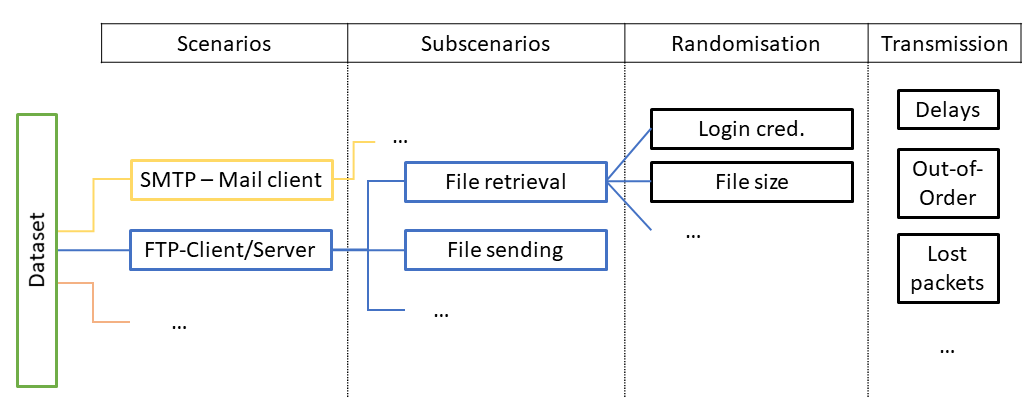
\includegraphics[width=0.480\textwidth]{images/scenario_branching.PNG}
 \caption{Visualization of the different levels at which traffic variation is introduced in DetGen.}
 \label{Fig:branching}
\end{figure}


\subsection{Scenarios and subscenarios}
\label{Sec:Scenarios}
Here we describe the design process of the scenarios, just like in the previous paper.

\subsubsection{Randomization}\label{Sec:randomsubscen}
\dots \dots

\dots \dots

\dots \dots
\subsubsection{Network transmission}\label{Sec:Netrand}
\dots \dots

\dots \dots

\dots \dots

\subsubsection{Implementation Process}
\dots \dots

\dots \dots

\dots \dots

\subsubsection{Attack generation with Metasploit/Metasploitable}
\dots \dots

\dots \dots

\dots \dots
 
%\subsection{Implemented scenarios}\label{Sec:ExistScen}


%\begin{figure}%[h!]
%\centering
%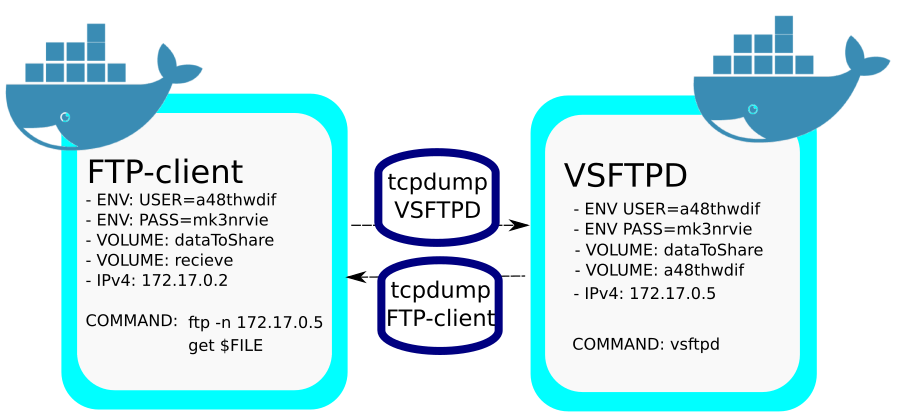
\includegraphics[width=0.49\textwidth]{images/ftp_new1.png}
%\caption{Diagram of FTP scenario}
%\end{figure}


\subsection{Network-emulation}

Describe the design of how the topology is generated before the data capture is started, and how the scenarios are launched and stopped during the data capture.
\subsubsection{Topology generation}
\dots \dots

\dots \dots

\dots \dots
\subsubsection{Launch-script}

\dots \dots

\dots \dots

\dots \dots

\subsubsection{Dataset coalescence}\label{Sec:datasetcreation}
\dots \dots

\dots \dots

\dots \dots
\subsubsection{Activity timeline input}
Here, we describe how the activity timeline in the launch script can come from unsophisticated distributions that we include, or from sophisticated 3rd party models such as Doppelganger. Since the modelling of computer activity is a field of ongoing research, it seems best to shift the responsibility for realistic models away by allowing this input. 

\subsection{Microservice-emulation mode}

\dots \dots

\dots \dots

\dots \dots


\section{Fidelity confirmation experiments}\label{Sec:Experiments}

This section is important to demonstrate that our data is valid and overcomes the difficulties entailed with synthetic data generation. Cordero et al. have proposed some more simple test that we can refer to first

\textcolor{red}{Question to be answered}: What requirements are there for the additional data, program logs and system logs, that we collect? Should we put less emphasise on these data sources in general if we are not able to perform these tests, and refer to them in future work? I am not aware of any papers that discuss these requirements in a similar way. 


\subsection{Data correctness tests}

This section is concerned with dataset defects, artifacts, or invalid data (inconsistent MTU etc.). These are very straightforward to test and should not take up much space. 


\subsection{Diversity tests}

These tests, also from Cordero et al. quantify diversity via the entropy of different quantities such as IP diversity, Time-to-Live, Maximum-segment-size, Window size, ToS. I think we should keep this relatively short and omit comparison to other datasets since this is already done by Cordero et al. 


\subsection{Structural dataset dimensionality}



Autoencoders are often used to compress non-deterministic, noisy data. Bahadur et al. have developed a procedure to estimate the ,,dimensionality'' (to be understood as the complexity) of a dataset using variational autoencoders. I believe we can transfer this concept to sequence compression and estimate the overall complexity of connection sequences in our framework with both real traffic captures and existing network intrusion datasets. 

Showing that our data is closer to real-world data would be a good test for "artificially predictable patterns", as described by Cordero et al., and go hand-in-hand with demonstrating the benefits of our framework for the training of deep-learning models. The importance of data that is less artificially predictable and closer to real-life traffic in terms of statistical variations lies in its suitability as a benchmark for detection rates, since less complex data is easier to train on and yields unrealistically high detection rates. 


%Measure structural richness of
%Also measure divergence across same activities (same activity and same port)
%Demonstrate benefit of structural richness
%Closer to reality



%\subsection{Reproducible scenarios}\label{Sec:deterministic}

%\dots \dots

%\dots \dots

%\dots \dots
%\begin{figure}
%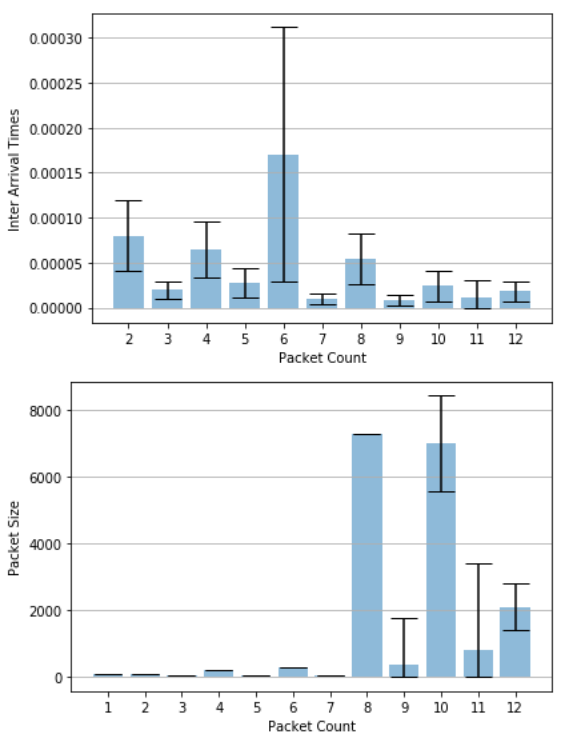
\includegraphics[width=0.45\textwidth]{images/combined3.png} % first figure itself
%\caption{Means of IATs \& packet sizes along with standard deviation bars for the first twelve packets in the Apache scenario.}
%\label{fig:size1}
%\end{figure}

 


% Need to edit these sections to provide a single context for both the artificial delays & classification

\subsection{Explorating Artificial Delays}

This section is already existing, we could potentially expand this. I think it is sufficient and analysing it more does not add much to the paper as the performance of TC netem is relatively well accepted. I think we could even move this section to the appendix.

%\begin{figure}
%\captionsetup{justification=centering}
%\centering
%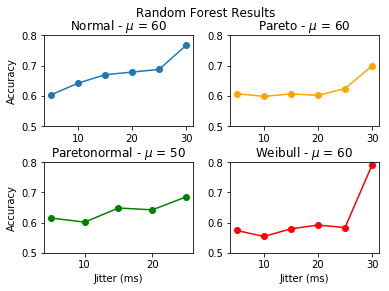
\includegraphics[width=0.45\textwidth]{images/1-plot_exp1.png}
%\caption{Results of Random Forest Classifier for a given distribution at the best performing delay mean $\mu$. Note that a score of .5 indicates total indistinguishability.}
%\label{Fig:rf_graph}
%\end{figure}
%
%
%
%\begin{table}[ht!]
%\begin{center}
%\begin{small}
%\begin{sc}
%\begin{tabular}{ccccc}
%\hline
%Distribution & Mean & Jitter & RF Accuracy\\
%\hline
%No Delays (Baseline) & 0 & 0ms & 0.8176 \\
%Constant Delay & 40ms & 0ms & 0.6730 \\
%Normal & 60ms & 5ms & 0.6028 \\
%Pareto & 60ms & 10ms & 0.5979 \\
%Paretonormal & 50ms & 10ms & 0.6015 \\
%Weibull & 60ms & 10ms & 0.5540 \\
%\hline
%\end{tabular}
%\end{sc}
%\end{small}
%\caption{Worst Random Forest accuracy rates for a given distribution}
%\label{tab:results-iat_rf}
%\end{center}
%\vskip -4mm
%\end{table}



\section{Use-cases}


\subsection{Benefits of ground-truth labels/dynamic dataset generation}
Possible title: \textbf{Dataset tuning to decrease false-positives}

Extensive ground-truth labels for our activities are arguably the most important contribution of the DetGen framework, so we should highlight their benefit most. Since ground-truth labels on attack data are existing in other datasets, we should emphasise the benefit of having labels for different activities. In my eyes, the most striking benefit arises for false-positive analysis, which we could then combine with showcasing the benefit of being able to generate different amounts of traffic for different activities.


\paragraph{Plan}
Implement the LSTM-model in the paper "An LSTM-Based Deep Learning Approach forClassifying Malicious Traffic at the Packet Level", train it on our data (both benign and attack traffic). Extract labels of traffic responsible for false-positives, show how much they are clustered around particular activities (potentially rare activities) compared to the overall traffic. Give potential reason for this. Generate a new dataset with increased amounts of the activities responsible for false positivies. Demonstrate that false-positives decrease.

\subsubsection{Benefits of structural richness}

Possible title: \textbf{Harder benchmarks}

As described above, the importance of data that is less artificially predictable and closer to real-life traffic in terms of statistical variations lies in its suitability as a benchmark for detection rates. In particular, we want to demonstrate that our data functions is a more difficult and realistic benchmark that is less prone to inflating detection rates than existing datasets, something that is often a point of criticism for models evaluated on synthetic data. 

To show that the training and detection is harder on our data, we could generate a dataset with similar attacks and services as the CICIDS-17 dataset, and train the above described LSTM model on both datasets. We could show that the training loss goes down more slowly on our data, as well as other metrics (increased validation loss --> overfitting etc.). We could then go ahead and show that the same attacks are detected easier by the same model in the CICIDS-17 data than in our data, concluding that it is a less realistic benchmark.

It would be good to also include a comparison with actual real-world traffic here to bolster our conclusion, but due to the lack of structured real-life datasets it is difficult to create a fair and scientific comparison. 

%\subsubsection{Show utility of tuning amount of rare events}

\subsection{Show utility of flexible topology}

This is another possibility to demonstrate that the flexibility provided through containerisation allows for better benchmarking and more in-depth evaluation.

Methods aiming at modelling network structures are an established method for botnet and pivoting detection. Even though the network topology is a crucial variable in their training, their evaluation is to my knowledge only done on single static datasets such as the LANL-15. 

My idea is that we generate about 10 datasets with different topologies, (especially different numbers of subnets and servers), and highlight the variation in prediction accuracy, i.e. the accuracy on one dataset is significantly higher/lower, and the average across the different datasets is a better indicator that eliminates the topology as a variable. We do not necessarily need to implement any attack traffic here since the modelling accuracy on benign traffic should be sufficiently quantifiable. 

A suitable candidate for the evaluation would be the paper "Link prediction in dynamic networks using randomdot product graphs", which comes from people at Imperial College that I know. The model tries to give a probability for each connection to appear in a network, in order to spot connections between unlikely pairs as anomalous behaviour. I could ask the people for the implemented model so we do not have to do it ourselves, or we could even have a chat with them.


%\begin{figure}%[ht!]
%\subfloat{%
% 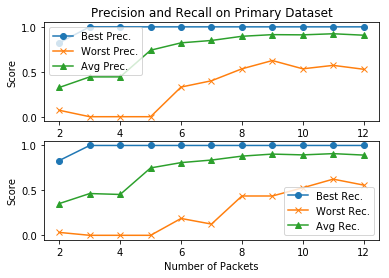
\includegraphics[width=0.4\textwidth]{images/bw_100_exp_3.png}}
%\subfloat{
% 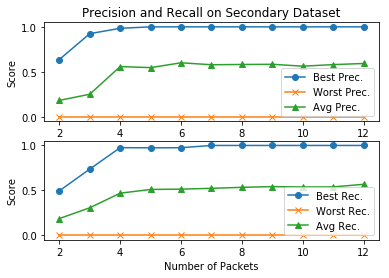
\includegraphics[width=0.4\textwidth]{images/bw_500_exp_3.png}}
%\caption{Results of Random Forest Classification on Primary dataset (Above) and Secondary dataset (Below)}
%\label{Fig:Primary}
%\end{figure}

\subsection{Customisable attack traffic by using metasploitable}

Rob and I discussed that by using a combination of a metasploit-attack container and a metasploitable-victim container, we could generate and embed a significantly larger number of attack traffic types more efficiently than we are currently. Since we can attach the metasploitable-container to the network interface of regular containers, we can embed the implemented vulnerabilities very easily in a given scenario. Furthermore, since both containers are well maintained, we can keep the attack catalogue up-to-date.

I think the best use-case is to showcase the process of adding a new type of attack to the dataset, embedding it in a proper way to a given scenario, generating data from it. We could additionally implement a corresponding detection method, but I think this would not demonstrate anything. 


\subsection{Simple use-case for the microservice mode?}

\section{Conclusions}\label{Sec:Conclusion}



\subsection{Difficulties and limitations}


\subsection{Future work}



%Syslog logging driver
%add server to capture syslogs 

%https://docs.docker.com/config/containers/logging/syslog/


%We are grateful for our ongoing collaboration with our industry partners  on this topic area, who provided both ongoing support and guidance to this work. Discussions with them have helped reinforce the need for a better evaluation and understanding of the possibilities that new intelligent tools can provide.

%Full funding sources after currently blinded.

\bibliographystyle{ACM-Reference-Format}
 
\bibliography{DetGen_ext}

%\appendix

%\section{Protocol Coverage}

%We initially investigated the protocols and applications present in existing network traffic datasets. Our analysis includes CIC-IDS 2017 \cite{sharafaldin2018toward}, UNSW-NB15 \cite{moustafa2015unsw}, ICSX Botnet \cite{beigi2014towards} and Mawi \cite{fontugne2010mawilab}. We chose these datasets as they provide \texttt{.pcap}-files of their network traffic which enables us to more easily see what protocols are present. To do this, we used the Bro IDS tool to generate log files, listing the results in table \ref{tab:results-bro}.

%The protocols listed in table \ref{tab:results-bro} make up over 90\% of the benign traffic in these datasets. Moreover, although the ratio of protocols in datasets can differ significantly, we see some patterns: namely, protocols associated with general browser usage, such as HTTP, SSL, DNS, are the most common in each dataset. 

%\begin{table}[ht!]
%\begin{center}
%\begin{small}
%\begin{sc}
%\begin{tabular}{ccccc}
%\hline
%Protocol & UNSW-NB15 & ISCX & CIC-IDS 2017 & Mawi\\
%\hline
%HTTP & 196195 & 2372 & 276405 & 156179 \\
%SSL & 540 & 141 & 285760 & 591551 \\
%DNS & 372748 & 200009 & 1820105 & 1581858 \\
%X509 & 459 & 331 & 2758590 & Unknown \\
%FTP & 111685 & 1989 & 5540 & 278 \\
%SSH & 31320 & 434 & 5600 & 5503 \\
%IRC & 202 & 27 & 0 & Unknown \\
%SMTP & 44455 & 125 & 0 & 4601 \\
%\hline
%\end{tabular}
%\end{sc}
%\end{small}
%\vskip -2mm
%\caption{Bro Log Flow Count}
%\label{tab:results-bro}
%\end{center}
%%\vskip -4mm
%\end{table}



%We could base the ratios of protocols in our own dataset off of those found in an existing dataset where the traffic has been artificially generated. However, this would be problematic. In the case of CIC-IDS 2017, some protocols that make up a substantial amount of real-world traffic are glaringly omitted, such as BitTorrent or video streaming protocols. In contrast, although UNSW-NB15 contains a better range of protocols, only a small percentage of their web traffic is transmitted over SSL which is unrepresentative of real-world traffic. Furthermore, in both these datasets, it appears that a non-negligible amount of traffic is the result of remote desktop protocols being used to interact with the virtual machines generating data, such as X11, VNC and RDP, which we consider to be unwanted noise. Instead, we opt to use these datasets as a rough guideline for constructing datasets but not closely following any one in particular.

\end{document}
